% Monte-Carlo-simulations.tex
% Topic: Monte Carlo Simulations
% (Advanced topic — outside the HSC Mathematics Extension 2 syllabus)

\textbf{Monte Carlo simulation} is a computational technique that uses random sampling to approximate numerical results. It is particularly useful when a problem is too complex to solve analytically.

\textbf{Basic idea:}
\begin{enumerate}[leftmargin=*]
  \item Define a random experiment whose outcome is related to the quantity you want to estimate.
  \item Simulate the experiment a large number of times (e.g.\ $N = 10{,}000$ trials).
  \item Estimate the quantity as the proportion (or average) of the simulated outcomes.
\end{enumerate}

\textbf{Estimating $\pi$ by Monte Carlo.} Consider a unit square with an inscribed quarter-circle of radius $1$.
\begin{itemize}[leftmargin=*]
  \item Generate $N$ random points $(x_i, y_i)$ with $x_i, y_i \in [0,1]$.
  \item Count the number $M$ of points satisfying $x_i^2 + y_i^2 \leq 1$.
  \item Then $\pi \approx 4M/N$.
\end{itemize}

\begin{center}
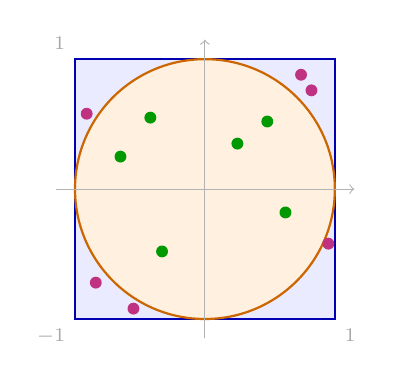
\begin{tikzpicture}[scale=1.65]
  % Square [-1,1] x [-1,1]
  \fill[blue!8] (-1,-1) rectangle (1,1);
  \draw[thick,blue!70!black] (-1,-1) rectangle (1,1);
  % Unit circle x^2 + y^2 <= 1
  \fill[orange!12] (0,0) circle (1);
  \draw[thick,orange!80!black] (0,0) circle (1);
  % Points inside the circle (x^2+y^2 <= 1)
  \foreach \x/\y in {0.25/0.35, -0.42/0.55, 0.62/-0.18, -0.33/-0.48, 0.48/0.52, -0.65/0.25}%
    \fill[green!60!black] (\x,\y) circle (1.3pt);
  % Points outside the circle (x^2+y^2 > 1)
  \foreach \x/\y in {0.82/0.76, -0.91/0.58, 0.74/0.88, -0.84/-0.72, 0.95/-0.42, -0.55/-0.92}%
    \fill[magenta!75!black] (\x,\y) circle (1.3pt);
  % Axes (optional thin guides)
  \draw[->,gray!60,thin] (-1.15,0) -- (1.15,0);
  \draw[->,gray!60,thin] (0,-1.15) -- (0,1.15);
  \node[below left,font=\scriptsize,gray!70] at (-1,-1) {$-1$};
  \node[below right,font=\scriptsize,gray!70] at (1,-1) {$1$};
  \node[above left,font=\scriptsize,gray!70] at (-1,1) {$1$};
\end{tikzpicture}\\[0.35em]
{\small
\textcolor{green!50!black}{$\bullet$} inside disk ($x^2+y^2\le 1$)\quad
\textcolor{magenta!75!black}{$\bullet$} outside disk ($x^2+y^2>1$)\quad
square $[-1,1]^2$ \textcolor{blue!70!black}{(blue)}, circle \textcolor{orange!80!black}{(orange)}.}
\end{center}
\noindent\textit{The diagram uses the full disk in $[-1,1]^2$; sampling only $[0,1]^2$ as above is the first quadrant of the same setup, with hit probability $\pi/4$.}

\textbf{Why it works.} The probability that a random point in the unit square lies inside the quarter-circle is $\pi/4$, since the area of the quarter-circle is $\pi/4$ and the area of the square is $1$.

% Placeholder: further examples and simulations to be added.
